% Literature review for the first meeting

\documentclass[a4paper,11pt,twoside]{article}
\usepackage[T1]{fontenc}
\usepackage[utf8]{inputenc}
\usepackage{color,dcolumn,graphicx}
\usepackage{wrapfig}
\usepackage[top=2.5cm, bottom=2.5cm, left=2.5cm, right=2.5cm]{geometry}
\usepackage{setspace}
\onehalfspacing
\usepackage{scrextend}
\addtokomafont{labelinglabel}{\sffamily}
\usepackage[english]{babel}
\usepackage[style=texConf/ele,maxcitenames=2,uniquelist=false]{biblatex} %
\addbibresource{/users/wvieira/Documents/mendeley_bibtex/Thesis.bib}% Syntax for version >= 1.2
\usepackage{tcolorbox}
\usepackage{filecontents}
\usepackage{csquotes}
\usepackage{epigraph}
\usepackage{ragged2e}
\usepackage{wrapfig}
\usepackage{authblk} %filiation
\renewcommand\Affilfont{\itshape\small} %filiation small %add logo before title
\usepackage[font=small]{caption}
\usepackage{hyperref}
\hypersetup{
  colorlinks = true,
  allcolors=[rgb]{0,0.4,0.5},
}
\usepackage{flafter} %make sure that the floats are not placed before their definition

%% Packages for Graphics & Figures
\usepackage{graphicx} %%For loading graphic files
\usepackage{float}

%% Math Packages
\usepackage{amsmath}
\usepackage{amsthm}
\usepackage{amsfonts}


\title{
  PhD project \\
  \bigskip
  Linking forest management and species distribution models: \\
  a theoretical approach under climate change
}

\author[1,*]{Willian Vieira}
\affil[1]{Département de Biologie, Université de Sherbrooke, Sherbrooke, Québec, Canada}
\affil[*]{w.vieiraw@gmail.com}
\date{}

\begin{document}

\maketitle

\begin{abstract}

\textbf{TODO}: \\
- Forest productivity \\
- Theoretical approach (SDM, resilience calculus, alternative stable state and early warning signals) \\
- All study case: Québec Forest resource \\
- All methods \\
- Better description of thesis structure \\
- Abstract \\
- Short reference style \\
- Change \LaTeX color syntax in Atom

\end{abstract}

%logo
\vfill
\begin{figure}
\centering
\includegraphics[width=16cm]{img/logo.pdf}
\end{figure}
\thispagestyle{empty} %no page number in the first page
\clearpage

\thispagestyle{empty}
\tableofcontents
\clearpage

% START DOCUMENT

\begin{displayquote}
\centering\textit{Ecology may provide many of the answers — but only if it is holistic enough to incorporate the human element as part and parcel of the ecosystem.} \\ \RaggedLeft{\parencite[p. 231]{Pfister1993}}
\end{displayquote}

\section{Context}

Climate change is an increasing trending topic in both non-scientific \parencite{Capstick2015} and scientific environment (Figure \ref{fig:fig1}), transforming our world as a metamorphosis of practice and acting \parencite{Beck2016}.
In the holocene epoch, the world's climate has never been completely stable, mainly impacted by different forces as, e.g., orbital, solar and volcanic \parencite{Wanner2008}.
However, in the last 200 years humans activities are contributing to increase the concentration of greenhouse gases, which can lead to increase the mean temperature, changes in precipitation patters and the strength of extreme climate events \parencite{Cubasch2013}.
These changes on climate are not only impacting the functionality of ecosystems and their capacity to provide essential ecological services for human well-being \parencite{Cardinale2012}, but also (surprisingly) the risk of death in humans \parencite{Mora2017}.

\begin{wrapfigure}{r}{0.38\textwidth}
    \centering
    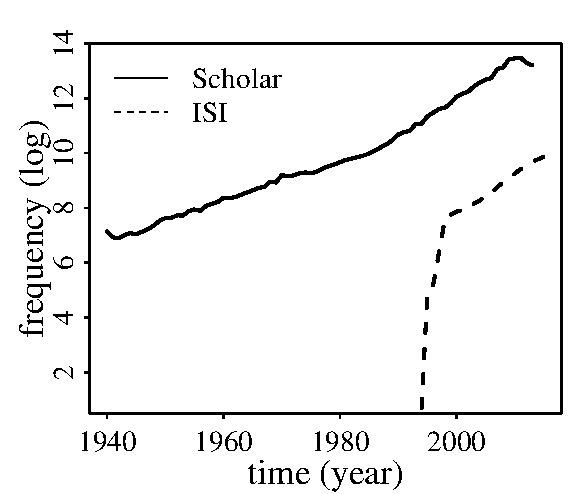
\includegraphics[width=0.38\textwidth]{img/fig1_em.pdf}
    \caption{Frequency of the keyword ``Climate change'' used in publications indexed on Google Scholar (1940 - 2013) and Web of Science (1994 - 2015)}
    \label{fig:fig1}
\end{wrapfigure}

Recent global changes have an impact on different biological mechanisms and an immediate key question is to understand the patters of this process.
Impacts of climate change go from local species constraints \parencite[e.g. low regeneration;][]{Treyger2011}, shift in species' range \parencite{Boisvert-Marsh2014,Monleon2015} and in community composition \parencite{Dieleman2015}, to range retractions and extinction \parencite{Thomas2006}, modifying biodiversity in all scales \parencite{Penuelas2013}.
To understand this link, climate variables are often used as predictors of trees site occupancy \parencite{Canham2010} and range limits \parencite{Morin2015}, in which, modeling approach projects a range shift to both higher elevations and higher latitudes under climate change \parencite{Chen2011}.

Species distribution models (SDM; defined in section \ref{sdm}) is one of the most popular method to predict species' range shift under climate change, providing a wide range of applications, as in biodiversity conservation and management \parencite{Guisan2005,Guisan2013}.
However, these models are generally phenomenological and  distributed at equilibrium with climate \parencite[e.g.][]{Pigot2013}, being an issue when species observation does not reflect its niche \parencite{Schurr2012}.
Furthermore, they do not consider important determinants of range limits as demography \parencite{Louthan2015}, ecological constraints \parencite{Wisz2013,Pigot2013} and species absences data \parencite{Koshkina2017}, inducing non-accurately projection of the future spatial distribution of a species \parencite{Tavecchia2016}.
Considering this determinants, trees' migration rate following climate change will be slower than predicted \parencite{Bertrand2011,Sittaro2017}, increasing the climatic debt \parencite{Bertrand2016}.

%Extinction debt is following climate debt?
The climatic debt is a measure of the lag (or disequilibrium) of plant communities with climate change, integrated in an environmental context \parencite{Bertrand2016}.
\textcite{Essl2015} has listed twelve mechanisms that contribute to delayed biodiversity responses, among them, changes appears at ecosystem (loss and degradation), community (secessional, biotic interaction, species removal and invasion) and population (evolutionary and adaptive) levels.
Physical changes cause biotic changes that directly and indirectly promotes species' persistence and/or species' migration \parencite{Bertrand2016}.
This mechanisms of persistence (measured by resistance) and migration (measured by recovery) leads to a climate debt and migration credit, respectively \parencite{Bertrand2016} but also a concept of resilience\footnotemark{} \parencite{Oliver2015}.
Therefore, climate lag promotes extinction debt (temporarily persistence of population under unsuitable conditions) and colonization credit \parencite[suitable locations are not occupied due species constraints;][]{talluto2017}, being a challenging for biodiversity conservation \parencite{Kuussaari2009} and productivity \parencite{Lasch2002}.
Identify the mechanisms shaping delayed biotic response of systems to environment, its resilience as well as alternatives to mitigate ecological constraints, is crucial to access the vulnerability of biodiversity to climate change and improve forecasts and biodiversity management \parencite{Essl2015,Oliver2015,Bertrand2016}.

\footnotetext{Here I use \textbf{recovery resilience} (recovery time to equilibrium) and \textbf{resistance} to describe the whole mechanisms of ecological resilience (see why in section \ref{res})}

\section{Preliminary objectives}\label{obj}
%I call this section as ``preliminary'' because I am still trying to figure out possible gaps I will be interested in working on.
%I also believe that classifying my plan as preliminary will help me identify throughout my thesis the ``best'' route to finish it in a pleasurable and creative way.

The primary objective of my thesis is to study if forest management can increase the speed of transition (i.e. recovery resilience) from temperate to boreal forests observed in the North Eastern America.
To achieve, I will use theoretical models parameterized from a forest inventory database, focusing on tracking uncertainty using Bayesian approach.
As an outcome, I will create a decision make tool to improve management strategies that take climate change into account.

During these first few months of reading, I asked myself the following questions that may direct my PhD: \\
(i) Which mechanisms are affecting the delayed biotic response to climate change? What is the origin, direction and intensity of these mechanisms? \\
(ii) How can forest management affect these mechanisms to increase resilience and therefore speed up the response? \\
(iii) What if we consider demography patterns, species interaction and natural disturbance in both local and global scale models? \\
(iv) Which role plays the interaction of forest management, climate change and disturbance on provision of ecosystem services? Which scale is the most important? \\
(v) How can the mechanisms we will find be used to inform applied management to enhance the resilience and productivity?

\section{Mechanisms of delayed biotic response}

Mechanisms shaping delayed biotic response and ecological resilience act at different scales and usually they interact with each other across scales, which makes the process sometime difficult to track and therefore to mitigate.
Furthermore, there is a focus attention in mechanisms at the metapopulation level where local mechanisms are often ignored \parencite{Hylander2013}; it creates a knowledge gap in understanding all the possibles mechanisms as well as its interactions.
In this context, I will start my thesis trying to identify how we can increase forest resilience by managing these mechanisms, or more specific, how to decrease the recovery time of a system from a disturbance to a steady state (theories described in section \ref{ta}).
Here, I present some mechanisms that may be affecting the delayed response to climate change, as well as forest resilience, in which may become possible topics I will be testing during my thesis using SDM approach, working both at local and large scale.

\subsection{Biotic Mechanisms}

Biotic mechanisms change the response from individual and population species to community level.
At the individual scale, the lifecycle elements of any species, represented by demography patters, is a mechanism able to alter the time response from environmental perturbations \parencite{Bertrand2016}.
For example, species with a high growth rate will recover faster \parencite{Grman2010}, in which we can expect a high recovery resilience; the allee effect can, however, induce the opposite effect by reducing mean vital rates \parencite{Dennis2002}.
In parallel, the sensitivity of a species also plays an important role in its response to perturbations \parencite{Oliver2015,Bertrand2016}; sensitive species respond faster and also has a high recovery resilience.
Alternatively, both species (with high growth and sensitivity) have a low resistance to environmental changes; it means that, if they have a low adaptive phenotypic plasticity, they will not be able to survive.
Phenotypic plasticity is the (behavior, morphology or physiology) change of an individual in response to the environmental change \parencite{Price2003}; this adaptive process, together with evolutionary adaptation \parencite{Bertrand2016} are mechanisms that increase both species resistance and recovery resilience \parencite{Essl2015,Oliver2015}.

In a metapopulation level, high genetic variability increase both resistance and recovery resilience of species \parencite{Hylander2013,Oliver2015}.
Dispersal mechanisms can affect genetic variability (the low exchange between individuals, the low variability), in which together with the low dispersal ability of forest species, can lead to an increase in climate debt \parencite{Hylander2013,Bertrand2016}.
Dispersion itself is a key mechanisms that can increase range shift under climate change \parencite{Gonzalez-Varo2017}. Yet, this mechanism is poorly supported by data; alternatively, species’ demographic rates are sufficient to predict population spread when dispersal data is absent \parencite{Hemrova2017}.
In addition to dispersion, the effective population size also affect genetic variability \parencite{Oliver2015}, where small populations increase the likelihood for inbreeding and hence the extinction risk \parencite{Nieminen2001}.
These individual and populational mechanisms are, however, rarely affecting species alone; instated there must be interactions between them \parencite{Hylander2013}, as well as extra mechanisms acting from different scales and origins.

Because different species are normally distributed together limiting one another \parencite{Clark2014a}, consider biotic interactions across trophic levels is essential to predict species distribution \parencite{VanderPutten2010}, as well as understand its impact on delayed biodiversity response \parencite{Essl2015}.
For instance, trees competition for soil nitrogen has amplified climate debt, but it varies depending on the resource \parencite{Bertrand2016}.
Generally, species interaction itself is determined by multiple mechanisms \parencite[for an overview]{Louthan2015} and a shift from single-species distribution to community distribution is suggested \parencite{Cazelles2016}.
In interaction networks, the loss of one specie can lead to cascade extinction, reducing the network stability \parencite{Dunne2002} and, if the specie is sensitive, the functional resistance.
In addition, the recovery resilience and resistance of a system depend if different species perform complementary functions (i.e. functional redundancy) or respond in different ways to perturbation \parencite{Winfree2009}; it means resistance increase when the network are dominated by non-specialized interactions \parencite{Oliver2015}.

\subsection{Abiotic Mechanisms}

Abiotic or physical mechanisms can also shape delayed biotic response and ecological resilience, in which a better quality environment will support plant development and therefore its resistance to perturbation.
At the soil level, for example, nitrogen availability can limit the growth of trees \parencite{Sullivan2013} and high nitrogen content and low acidity soils impact both species sensitivity and competition, amplifying the climate debt \parencite{Bertrand2016}.
Likewise, less suitable climates constrained demographic strategies, increasing retrogression and vulnerability of plant species \parencite{Csergo2017} and increase the severity of climate events, inflating climate debt \parencite{Bertrand2016}.
In contrast, warming temperatures and higher CO2 concentration did not amplify ring growth \parencite{Girardin2017}.

Because environmental heterogeneity increases overall species richness \parencite{Stein2014}, the resistance of a system is enhanced by functional redundancy \parencite{Oliver2015}.
Environmental heterogeneity also provides a range of microclimatic refugia, which allow species to persist locally to climate changes \parencite{Maclean2015}; however, \textcite{Bertrand2016} found that microclimatic refugia plays a minor role comparing with other determinants of climatic debt.
Ecosystem loss and degradation are mechanisms that contribute to loss and decrease in species diversity \parencite{Essl2015}, as well as decrease landscape connection.
Species in disconnected landscapes have then slow recovery resilience after perturbation, that is, low functional connectivity \parencite{Oliver2015}.

Disturbance can have different sources (natural or anthropic) and the response of forest to disturbance can be positive or negative (or even neutral) depending on the intensity of disturbance.
Natural disturbance are diverse and normally act quickly with high effect as, e.g., fire, flooding, pest outbreaks.
These disturbances are often negative as generate decline in species density, community richnesses and connectivity, in other words, reduce forest resilience \parencite{Buma2011,Essl2015} but see \parencite{Bertrand2016}.
However, according to the famous intermediate disturbance hypothesis, too little disturbance induces competitive exclusion and and too much disturbance long-lived species elimination \parencite{Grime1973,Horn1975,Connell1978}; which means that between extremes higher species richness is expected and hence higher forest resilience.
Human-induced disturbances is becoming increasingly frequent and, not surprisingly, climate change is one of the most important \parencite{Bellard2012}.
But beyond that, human's disturbance is present almost everywhere, from local impacts, as soil degradations, to global ones, as mining disaster \parencite{Garcia2017}; it implies that all mechanisms of disturbance, as well as its interaction \parencite{Goring2017}, has to be considered to a better understand of forest resilience and, hence, biodiversity management.

\section{Forest management}

Forest managers have an important (and challenging) mission to create strategies that will both adapt and mitigate forest under climate change \parencite{Millar2007}.
Mitigative practices are often addressed, forest management can affect carbon cycle and retention, hydrology dynamics and the maintenance of rich suitable habitats \parencite{Becknell2015}; however, adaptive ones are not that evident.
Currently, management practices are usually based in mechanisms of immediate action-effects and not in theoretical concepts; also, some factors are more amenable to manage (as e.g. genetic variability) than others \parencite[e.g. individual sensitivity, presence of alternative stable states;][]{Oliver2015}.
Therefore, a theoretical approach can improve our understand of forest management and help we move towards a more sustainable intervention.

Looking analytically, practices as plantation, cutting and pre-commercial thinning can be used to change the mechanisms of colonization, perturbation and succession, respectively (Figure \ref{fig:fig2}).
For example, plantation cannot just enhance colonization but also determine future forest structure by choosing what species to plant.
Similarly, reduce forest density by silvicultural thinning can enhance diameter growth \parencite{Rytter2014} [but depend on thinning intensity \parencite{Olivar2014,Fuller2013}], forest productivity \parencite{Chase2016a}, drought resilience \parencite{Bottero2017,Sohn2013} and accelerate succession; however, birds respond different to thinning and decrease in some species were observed \parencite{Hayes2003}.
Forest harvest can equally enhance disturbance and, by the fact that intermediate disturbance can enhance biodiversity \parencite{Grime1973,Horn1975,Connell1978}, the intensity and frequency of harvest can be important to decide whereas productivity will increase or not.

\begin{figure}
    \centering
    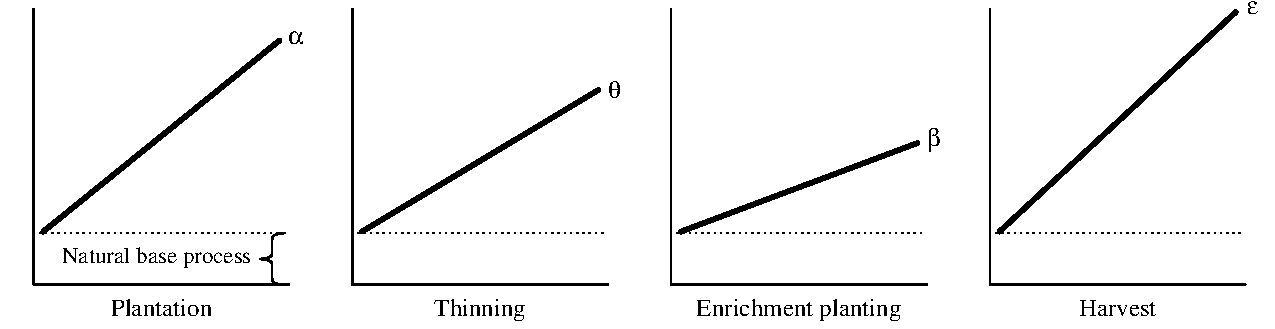
\includegraphics[width=1\textwidth]{img/fig2.pdf}
    \caption{Hypothesized interaction between forest management and state transition processes. Plantation can enhance colonization ($\alpha$), pre-commercial thinning can enhance both competitive exclusion ($\theta$) and succession ($\beta$) and cutting can enhance disturbance ($\epsilon$). Dotted line is the base natural process that occur without intervention.}
    \label{fig:fig2}
\end{figure}

In contrast, we cannot consider management as a single solution by the fact that managing practices can have different action depending on the context \parencite{Millar2007}, also external factors and interaction between practices can lead forest management to be complex \parencite{Becknell2015}.
For instance, theoretical methods, based in a macrosystem ecology approach, can access the interaction between forest management, climate change and disturbances to better provide ecosystems services \parencite{Heffernan2014,Becknell2015}.
Briefly, data synthesis can combine different methods as monitoring networks, remote-sensing, field studies and modeling to create an integrative approach able to evaluate forest change under different contexts \parencite{Becknell2015}.
Furthermore, ecological conditions, economic trends, policy and social priorities can influence forest management, where these practices vary in intensity, spatial extent and in frequency \parencite{Becknell2015}.

The adaptation process described above has two interpretations, the first one is a directed management to whereas the manager wants to go, mainly based in productivity of target species.  Instated, the second one is a natural adaptation, which includes acclimatization, ecological reorganization and evolution through natural selection \parencite{Webster2017}.
The Predict-and-prescribe approach aims to protect target species based in predicting future environmental conditions, however, the uncertainty of predictions still high, hence the effectiveness of this approach is limited \parencite{Schindler2015}.
Based on the portfolio theory, a successful approach happens when a diversity of portfolios environments, species, and communities promote a wide diversity of options, where in the end, nature is the one that peaks the ``winners'' \parencite{Webster2017}.

%\subsection{Ecosystem services provided by forest}
%
%Present the main services it could have (Becknell2015)

%\textbf{Forest productivity}.
%Timber buildings are getting safer, stronger and taller — and they could help to cool the planet. In why should we improve forest productivity
% http://go.nature.com/2rfsPy2

%Robert m'a envoyé quelques articles qui discutent des facteurs qui contrôlent la dominance des arbustes éricacées en forêt boréale et de leur possible impacte sur la productivité forestière.
%Lire toute le mail que je vais arriver avoir une bonne base pour discuter ici.

%paper:Temporal stability in forest productivity increases with tree diversity due to asynchrony in species dynamics

%Lasch et al. (2002) observed a productivity decrease in forest under climate change scenarios.

\section{Theoretical approach}\label{ta}

Read the section \textit{recent developments in predicting changes in species distribution} from \textcite{Ehrlen2015}

\subsection{Range dynamics theory}

What theories can help us to describe species range under climate change?\\
How to integrate forest management in this theory?\\
-> Metapopulation dynamics theory <-

\subsection{Resilience}\label{res}

A classical definition of resilience in ecology is the ability of ecosystems to absorb changes and still persist \parencite{Holling1973}.
The concept was further developed in other context (e.g. social-ecological systems), and a more contemporary definition considers resilience as (i) the amount of disturbance the system can absorb, (ii) the degree the system is able to self-organize and (iii) the degree of learning capacity to adapt to disturbance \parencite{Cumming2011}.
We have therefore two concepts, the time to \textbf{recovery} to stability and accommodated external changes \parencite{pimm1984,Folke2002} and the \textbf{resistance} of a particular ecological state to change \parencite{Peterson1998}.
Although \textcite{Oliver2015} treat both resistance and recovery as related aspects of resilience, I prefer to keep these concepts separated in (i) recovery resilience (or engineering resilience) and (ii) resistance where both are englobed in ecological resilience \parencite{Hodgson2015,Nimmo2015}.
Ecological resilience can be affected by different mechanisms from species to landscape levels, but biodiversity shows to be crucial to maintain long-term resilience of ecosystem services \parencite{Oliver2015}.

It is also important to not confuse recovery resilience with stability of a system.
Recovery resilience is the rate and extent of ``restoration'' of a system while stability is when the system maintains stable following small perturbations over time.
Before introduce the method to calculate recovery resilience, we must know what is the equilibrium and stability (\hyperlink{box1}{Box 1}) of a system, as well as these measures are relative and careful must be taken when choosing \textit{resilience of what to what} \parencite{Carpenter2001}.

\begin{tcolorbox}
\hypertarget{box1}{Box 1}. Equilibrium and Stability
\begin{align}
E &= mc^2 & \text{Formula of the universe}
\end{align}
\end{tcolorbox}

\begin{tcolorbox}
\hypertarget{box2}{Box 2}. Environmental transition (see Oliver2015)
\begin{align}
E &= mc^2 & \text{Formula of the universe}
\end{align}
\end{tcolorbox}

\textbf{(iii)} But how to calculate it in a analytical way?
To implement the results from these or other studies in management projects, it is necessary to disentangle the many meanings and measures of resilience and related stability concepts (In Mori at TREE).
Now introduce the calculus of $\lambda$ by Jacobian matrix (\hyperlink{box2}{Box 2}).
The Jacobian matrix has been used in different applications, from local models [...] to meta-ecosystems models \parencite{Gravel2016}

\subsection{Transition period - Alternative Stable States?}
The existence of single equilibria is still often assumed in the literature, with critical implications for conservation and restoration. -- An important feature of this concept (resilience) is the emphasis on possible alternative system properties that are associated with renewal and reorganization after disturbance (In Mori 2016 at TREE)

Resilience-based management does not typically seek to increase the rate of return to an original state, which often implicitly assumes the existence of a single equilibrium, but instead recognizes that many natural systems could have multiple attractors [2, 3]. (In Mori 2016 at TREE)

\subsection{Early warnings?}

Resilience indicators: prospects and limitations for early warnings of regime shifts

For precautionary biodiversity management, the identification of robust early-warning signals (e.g., critical slowing down of recovery rates after perturbations) of approaching thresholds (tipping points) of losses of biodiversity or ecosystem services [9] is urgently needed (in Essl2015)

\section{Study case: the Quebec forest resource}

Explain here where I am going to work and also why I am choosing this area.

May Robert's project help?!

Nice review about boreal forest in \parencite{Price2013}

\section{Methods}
Here we see a briefly presentation of possible methods will be used in the thesis.

\subsection{Modeling}

Why and how modeling?\\
Morin et thuiller 2009:{What then are the best strategies for obtaining accurate predictions for changes in the distributions of deciduous temperate trees? At the scale of the geographic distribution of species, no experiments in situ can be reasonably carried out to predict possible range shifts (Woodward 1987). Modeling therefore appears the most feasible and efficient way to establish useful predictions (Lovejoy and Hannah 2005, Thuiller 2007), and several kinds of models have been developed during the previous decade for this purpose. As reviewed by Midgley et al. (2007), these models fall into two main classes: vegetation-type models (dynamic global vegetation models [DGVMs]) and species-specific models (niche-based and process-based).}

 L’article de Ashraf et Maclean porte sur un modèle de simulation de croissance d’arbres individuels en fonction des changements climatiques.  Leur modèle a été développé avec une technologie d’intelligence artificielle.

\subsubsection{Species Distribution Models}\label{sdm}

Nice resume about SDM in \textcite{Moran-Ordonez2016}.


\subsubsection{Integral Projection Models}

the predictive powers of state and transition models are relatively low and their ability to deal with uncertainty is limited (Bashari, Smith and Bosch, 2008; Phillips, 2011).

\subsection{Bayesian approach}

\textit{I should be writing and not playing with \LaTeX}

\section{Thesis structure}

The first part of the thesis will be a general introduction where I will probably use a part of this document and present the big picture of my thesis.
I believe the introduction part of a thesis is an easy way to welcome the reader through my work, however in the actual context of digital era, no one really reads a whole PhD thesis.
An alternative approach to (sleepers) general introductions that, according to Stephen Heard\footnotemark{} no one reads but the author, is to publish it as a general papers in a scientific vulgarization journal.
In this way, my work will be easier to understand by both academics and general public, more accessible and the introduction part more useful.

The first chapter will try to answer the question \textit{How can forest management increase forest resilience to climate change?}.
The paper will work with a four states transition model and, by analytical analysis, we will try (i) to identify the most important mechanisms shaping transition processes, (ii) measure how can forest management change these mechanisms, and (iii) understand the impact of these changes on forest resilience.
Furthermore, as a study case in the North Eastern America forest, we will run simulations with the most effective management practices, found from the analytical analysis, under different scenarios of climate change.
We expect forest management to enhance recovery resilience by the hypothesis that plantation and thinning will increase colonization and succession (This chapter answers questions I and II from section \ref{obj}).

In the second chapter I will build a landscape Integral Projection Model (IPM) that will take forest management, species interaction and natural and human disturbance into account.
State and transition models has a low predictive power and limited ability to track uncertainty \parencite{Bashari, Smith and Bosch, 2008; Phillips, 2011}, IPMs are then an interesting alternative that can increase both of these weakness \parencite{}.
We expect... (This chapter answers questions III and IV from section \ref{obj}).

The third chapter I am going to build another model but in a local scale. \textit{I have to find a good biological reason for that}.

The fourth chapter will then integrate both landscape and local model into one. Here I will also track the uncertainty of the model by bayesian approach.

Finally, I will try to introduce my PhD reflexions into the big picture of ecology, management and ecosystem services. In an integrative and synthetic approach (more appropriate for a \textit{Forum} section), I will discuss my main results, its application and mainly the point of depart for future prosperous work. (This chapter answers question V from section \ref{obj}).

\footnotetext{The three functions of a thesis, by Stephen Heard at the \href{https://scientistseessquirrel.wordpress.com}{Scientist Sees Squirrel}'s blog}

\clearpage
\printbibliography

\end{document}
